\clearpage
\section{Resultater}

Vi skal nå se nærmere på Chad og Afghanistan som eksempler på land med
forskjellige antall og frekvens av hendelser. Chad er et land med mye 0-verdier
(høy $\hat{p_0}$). Afghanistan er i den andre enden av skalene med lav andel
0-verdier (lav $\hat{p_0}$). Begge landene viser overspredning i antall
dødsfall.. Videre vil vi vurdere modellene når man ser på alle landene under ett.
Vi har også sammenlignet modellene med en variant av en 0-modell, $Y_t|Y_{t-1}
= Y_{t-1}$. Det vil si en modell som predikerer at antall dødsfall i neste uke
er det samme som antall dødsfall i denne uken, en såkalt no change-modell (NC).

Sammenhengen mellom prediksjonener og observasjonene kan man se på
residualene. I \cref{fig:residuals_orig} er de ustandardiserte residualene
plottet for Chad og Afghanistan. Modellene overestimerer ved lave observerte
dødsfall og underestimerer ved høye observerte dødsfall. De standardiserte
residualene viser bedre hvordan de to fordelingene skiller seg fra hverandre
(\cref{fig:residuals}). For Afghanistan predikerer begge modellene ganske likt,
men LN-modellen underestimerer i større grad for de ekstreme verdiene. For Chad
har NB-modellen noe lavere standardiserte residualer en LN-modellen.  

Residualene alen er ikke nok for å bedømme modellene. I
\cref{tab:scoring_summary} vises den kvadrerte feilen og scoring rules. For
alle land sett under ett har LN-modellen lavest feil, det vil si prediksjoner
som er nærmest de observerte verdiene. For de normaliserte feilene er NB og
NC-modellene de som har lavest feil. For DSS og RPS ser man også at NB-modellen
gjør det bedre enn LN-modellen. No-change modellen sett over alle land lavest DSS-score.  

\begin{figure}[!h]
\centering
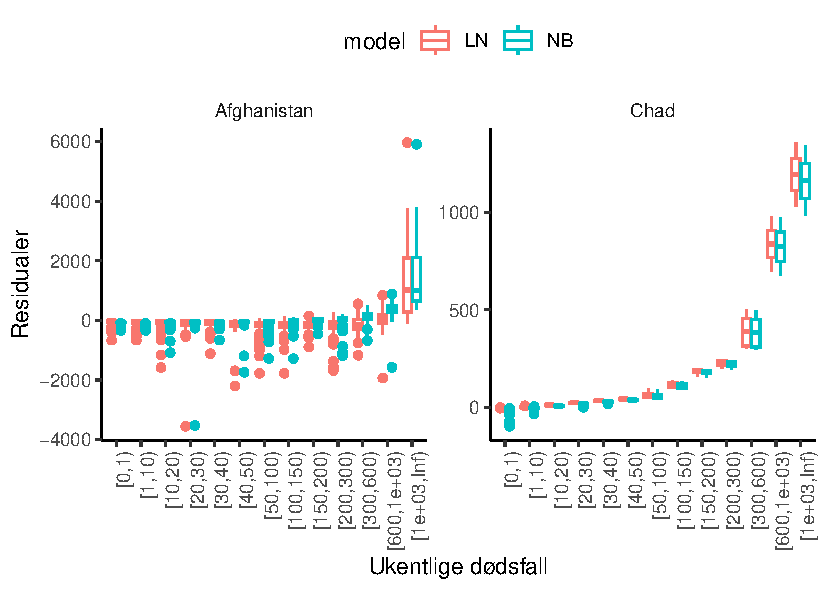
\includegraphics{../img/res_orig.pdf}
\caption{
    Antall dødsfall og residualer for Chad og Afghanistan.
    } 
\label{fig:residuals_orig}
\end{figure}

\begin{figure}[!h]
\centering
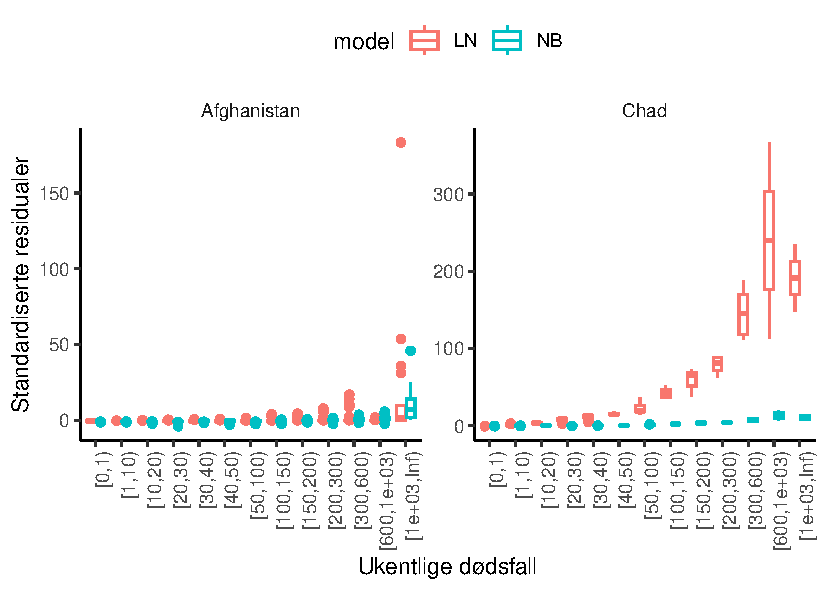
\includegraphics{../img/residuals.pdf}
\caption{Standardisert antall dødsfall og standardiserte residualer for Chad og
    Afghanistan. Antall dødsfall er standardisert ved å dele på variansen for
    landet.} 
\label{fig:residuals}
\end{figure}

I \cref{fig:pred_plot} vises prediksjonsintervallet for de prediktive
fordelingene gitt antallet dødsfall ved $t-1$. For Afghanistan har NB-modellen
et smalere intervall enn LN-modellen. For Chad har LN-modellen brutt sammen og
har mest vekt ved verdier nærme 0. LN-modellen ignorerer variasjonen i
observasjonene.  

\begin{figure}[!h]
\centering
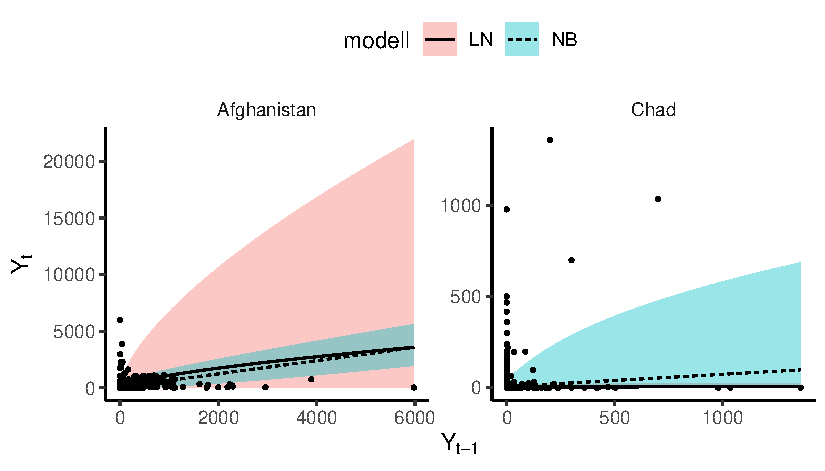
\includegraphics{../img/pred_plot.pdf}
\caption{
    Antall dødsfall ved $t-1$ mot antall dødsfall ved tid $t$. Et 95 \%
    prediksjonsintervall for hver av modellene er markert med henholdsvis rødt
    (LN) og grønt (NB). Forventningen er markert med hel linje (LN) og stiplet
    linje (NB). LN-modellen er så vidt synlig som et smalt bånd nederst.
} 
\label{fig:pred_plot}
\end{figure}

\begin{table}[!h]
\centering

\begin{tabular}[t]{llrrrr}
\toprule
Land & Modell & RMSE & RMNSE & DSS & RPS\\
\midrule
Afghanistan & LN & 178.39 & 0.54 & 36.18 & 94.56\\
Afghanistan & NB & 120.26 & 0.62 & 13.64 & 89.37\\
Afghanistan & NC & 120.23 & 0.34 & 12.76 & -\\
\addlinespace
Alle land & LN & 18.03 & 1.30 & 360.36 & 14.61\\
Alle land & NB & 19.38 & 0.40 & 10.51 & 14.14\\
Alle land & NC & 20.48 & 0.20 & 8.54 & -\\
\addlinespace
Chad & LN & 8.13 & 2.55 & 261.33 & 7.42\\
Chad & NB & 13.00 & 0.22 & 8.78 & 6.99\\
Chad & NC & 12.42 & 0.17 & 9.63 & -\\
\bottomrule
\end{tabular}
    \caption{Tabell over skåringsverdiene, RMSE og standardiserte RMSE
    (RMNSE), samt Dawid-Sebastini score (DSS) og Ranked Probability Score
    (RPS).}
\label{tab:scoring_summary}
\end{table}

\begin{figure}[!h]
\centering
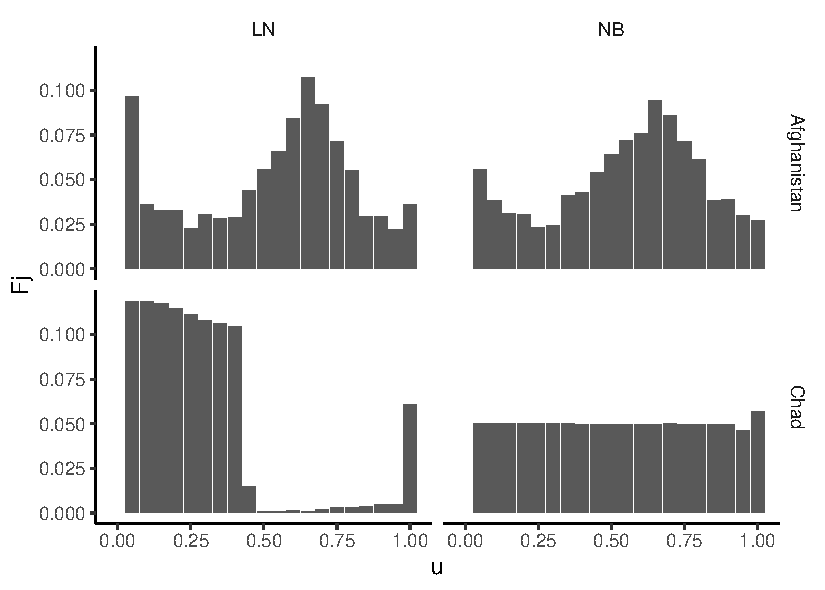
\includegraphics{../img/PIT_plot.pdf}
\caption{
    PIT-diagram for begge modellene for Afghanistan og
    Chad. 
}
\label{fig:PIT_plot}
\end{figure}

PIT-plottet (\cref{fig:PIT_plot}) viser at for Afghanistan er det overspredning
i de prediktive fordelingene. De høye søylene i PIT-plottet lognormal-modellen
i Afghanistan (øverste panel til venstre) er det antydninger til at det er noen
ekstremverdier som er større enn forventet ut fra modellen. For Chad er
forskjellen mellom modellene tydelige. Negativ binomialmodellen viser et flatt
histogram, noe indikerer fordelingen tilnærmer seg de observerte verdiene i
stor grad. Lognormal-modellen derimot har en prediktiv fordeling som tydelig har underspredning.  

For å si noen hvor de to modellene gjør det bra og hvor de bryter sammen har vi
plottet andelen 0-verdier mot feilen og DSS-score (\cref{fig:p0_plot}). For
RMSE ser vi at ved en andel 0-verdier over 0.7 er den RMSE lav. Den
standardiserte feilen RMNES er jevnt over lavere for NB-modellen jo høyere
andel 0-vedier. LN-modellen har større RMNES dess høyere andel 0-verdier. Det
samme mønsteret viser seg på DSS-score, med noen unntak hvor LN-modellen har
lavere score. Dette understøtter at LN-modellen legger mer vekt på 0-verdiene
verdiene på bekostning av å estimere variasjonen.


Videre har vi plotte spredningsindeksen $I_{\mathrm{disp}}$ mot RMSE, RMNSE og
DSS-score (\cref{fig:disp_plot}). RMSE øker for begge modellene når
$I_{\mathrm{disp}}$ øker. RMNSE øker for LN-modellen, men ikke for NB-modellen.
For begge modellene øker DSS-scoren med $I_{\mathrm{disp}}$, men mer for
LN-modellen.

\begin{figure}[!h]
\centering
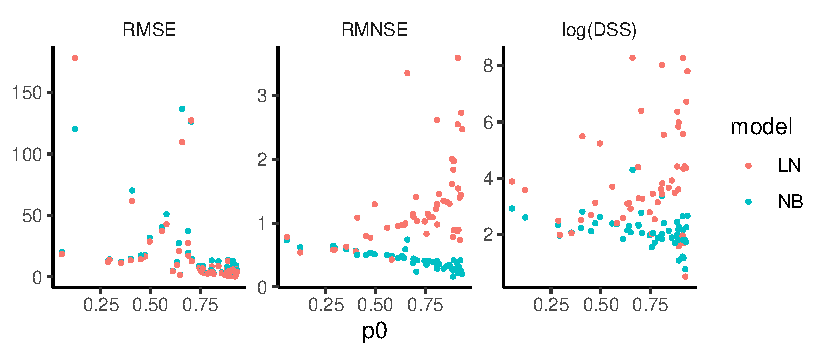
\includegraphics{../img/p0_plot.pdf}
\caption{
    Andelen 0-verdier plottet mot RMSE, normalisert RMNSE og log(DSS) for alle
    land for de to modellene.
}
\label{fig:p0_plot}
\end{figure}

\begin{figure}[!h]
\centering
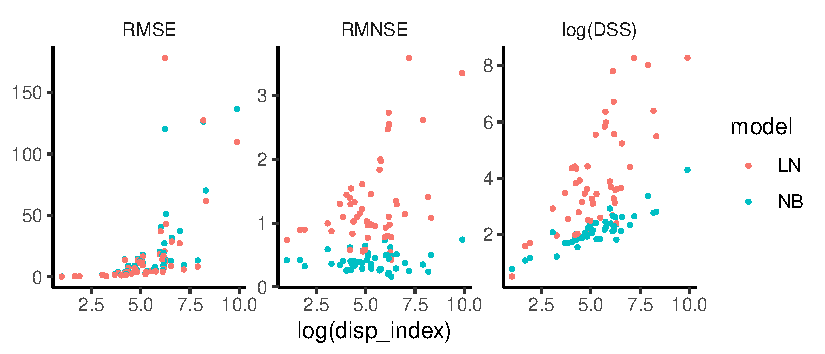
\includegraphics{../img/disp_plot.pdf}
\caption{
    Spredningsindeksen plottet mot RMSE, normalisert RMNSE og log(DSS) for alle
    land for de to modellene.
}
\label{fig:disp_plot}
\end{figure}

